% !TEX root = MutationTestingSurvey.tex

\section{Theory and Process of Mutation Testing}
\label{sec:process}

	\begin{figure}
	\centering
		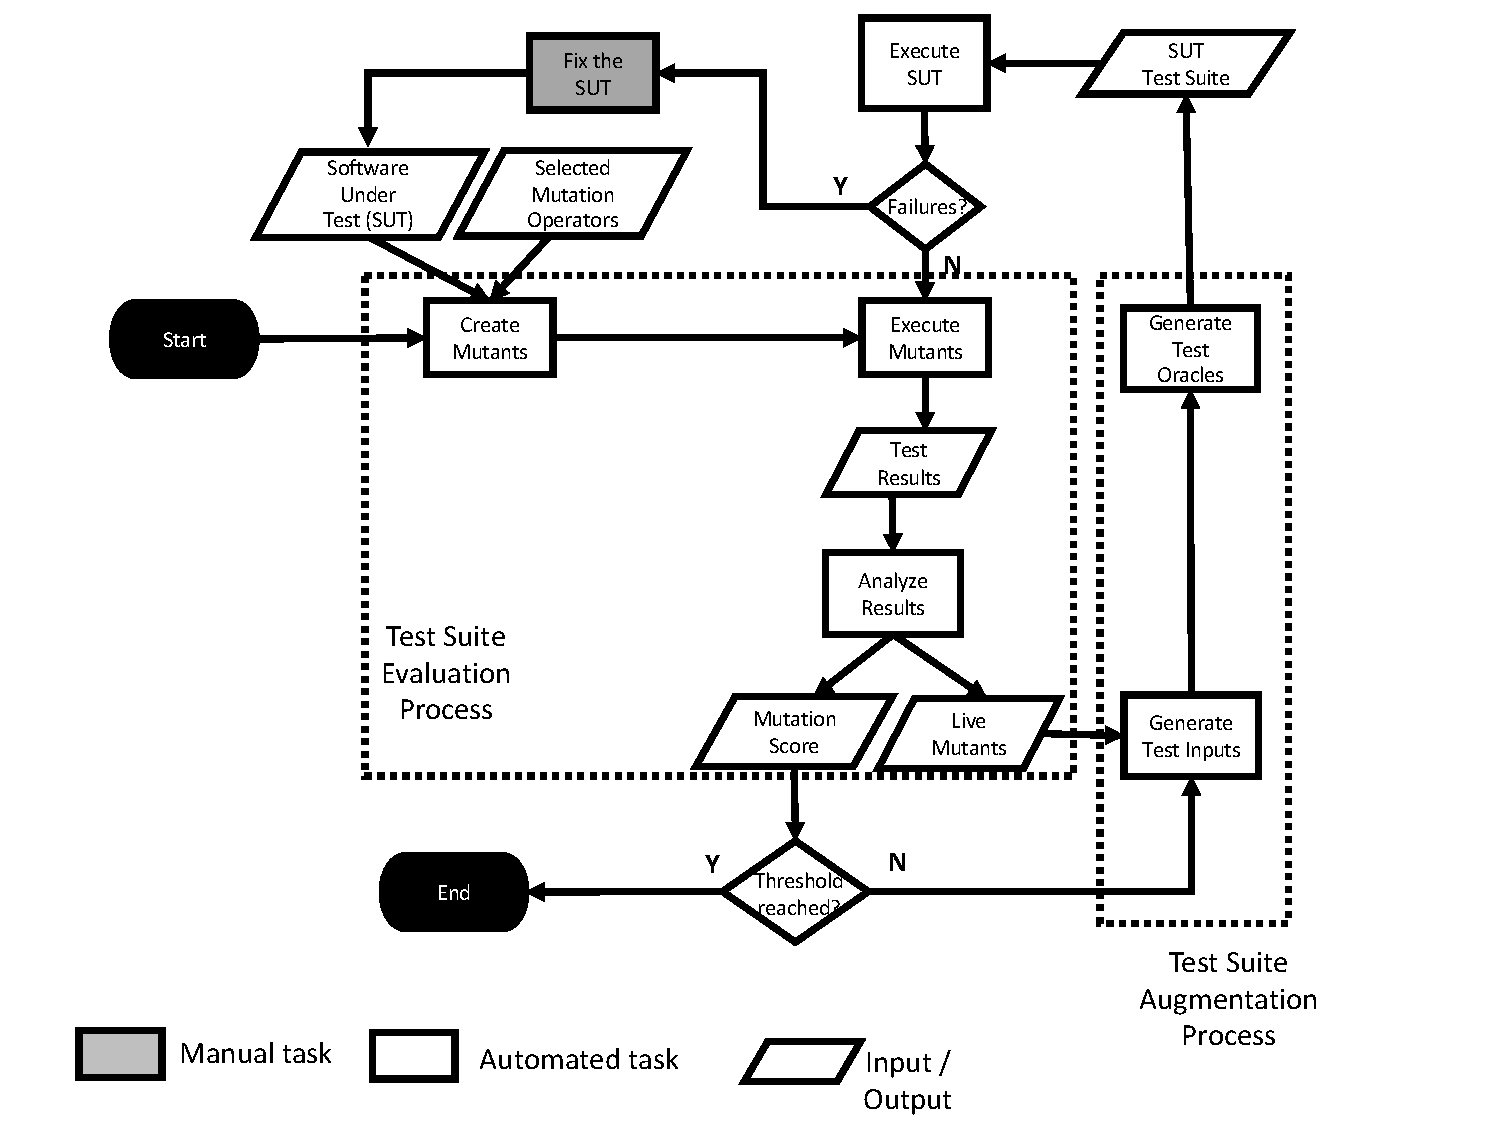
\includegraphics[width=\textwidth]{images/process}
		\caption{Mutation Testing Process.}
		\label{fig:process}
	\end{figure}

Figure \ref{fig:process} shows the reference code mutation testing process that will be considered in the survey. The process in Figure \ref{fig:process} has been inspired by the process mentioned in related work \cite{offutt2001mutation,papadakis2019mutation}. The process is based on two main sub-processes, Test Suite Evaluation and Test Suite Augmentation. The two sub-processes consist of multiple tasks which are generally automated by toolsets, in our context they will be automated by the FAQAS framework. 

\subsection{Test Suite Evaluation} % (fold)
\label{sub:test_suite_evaluation}

The Test Suite Evaluation process automatically generates modified versions (i.e., the mutants) of the software under test (SUT) and evaluates the quality of the SUT test suite by executing the test suite against all the mutants. Engineers provide the SUT and a selection of the mutation operators to consider. The set of mutation of operators to be applied depends on the implementation of the component that creates the mutants. A typical set of mutation operators implemented by most of the existing toolsets consists of the relational (ROR), logical (LCR), arithmetic (AOR), absolute (ABS) and unary insertion (UOI) operators \cite{rothermel1996experimental}. Several research paper target the definition of mutation operators; relevant for this ESA activity are works on the definition of mutants for floating point operators \cite{dan2012semantic}, operators synthesized by processing the revision history of C projects \cite{brown2017care}, mutation operators targeting memory operations \cite{wu2017memory}, deletion operators \cite{delamaro2014designing}, operators targeting components integration \cite{grechanik2016mutation}. Finally, recent attention has been put towards the development of higher-order mutation operators \cite{harman2010manifesto,ghiduk2017higher}. First order mutation seeds faults generated by a single syntactic change to the original program. Higher order mutation combines first order mutants to simulate more complex faults, motivated by a desire to capture subtle faults \cite{jia2009higher}.

In the mutation testing process, the automated application of the mutation operators to the source code of the SUT leads to the generation of modified versions of the SUT (i.e., the mutants) that should be compiled and then executed against the test suite to evaluate the test suite quality. Unfortunately, the mutation process leads to a high number of mutants to be generated, which leads to scalability issues due to the time required to compile and execute the dfferent versions generated. Recent surveys provide an overview of existing optimization techniques \cite{ferrari2018systematic}; the most relevant optimization approaches target the compilation processes, the execution of mutants, and mutants selection. To reduce compilation time, mutant schemata \cite{untch1993mutation} are adopted to encode all the mutants in a single file and parametrize the mutant execution so that mutants are compiled in a single pass and selected at runtime. The split-stream execution optimization consists of generating a modified version of the SUT that creates multiple processes (one for each mutant) only when the mutated code is reached \cite{tokumoto2016muvm}. With split-stream, the code shared among multiple mutants is executed only once thus saving time and resources. Other execution optimizations consist of minimizing the number of processes being created by sharing one single process among mutants that bring the system into the same state \cite{wang2017faster}.
Two main mutant selection approaches have been defined: the selection of mutation operators and the random selection of mutants \cite{zhang2010operator}. The first approach consists of the empirical identification of a subset of mutation operators that is sufficient to predict the mutation score \cite{siami2008sufficient,barbosa2001toward}. The second approach consists of randomly selecting a certain percentage of mutants from the generated ones \cite{wong1995reducing}, possibly with a uniform distribution of the different mutation operators \cite{zhang2010operator}. Empirical results with academic case studies \cite{zhang2010operator} show that the first approach is not superior to random selection when selecting the same number of mutants. Other work \cite{zhang2013operator} show that the combination of operator-based selection and random sampling leads to better results since it leads to high mutation score (above 98\%) while reducing the average mutation testing time to 6.54\%. The use of higher-order mutants is another solution to reduce the overall number of mutants. Other optimizations are framework specific, for example Mull limits mutations to reachable code \cite{hariri2018srciror}.
Another step of the mutation testing process is the identification of equivalent and redundant mutants. Equivalent mutants are mutants that behave as the original program, while redundant mutants are mutants that lead to the same erroneous program behaviour. Trivial compiler optimization is an approach that might be adopted in both the two cases and relies on the idea that source code that leads to the same program behaviour often belongs to the same optimized compiled code \cite{papadakis2015trivial}. Other approaches concern the adoption of symbolic execution \cite{papadakis2012mutation,kurtz2015static} and the runtime monitoring of the SUT (e.g., mutants that lead to the same execution paths are likely equivalent \cite{schuler2013covering}).
The execution of mutants simply concerns the execution of the test suite of SUT against the generated mutants, possibly with the optimizations reported above. In the case of a test failure, the SUT is expected to be fixed, otherwise engineers are expected to evaluate the quality of the test suite by observing the mutation score and inspecting live mutants (i.e., mutants that have not been killed). The mutation testing process terminates when a certain threshold for the mutation score is reached, otherwise the test suite should be improved. The computation of the mutation score is based on the percentage of mutants identified by test failures, i.e., based on difference between the expected and the observed output of the system. This approach is known as strong mutation coverage. Weak mutation coverage consists of verifying if the state of the system has been altered, with respect to the original code, after the execution of the mutated statement. Firm mutation coverage consists of verifying if the change in the state of the system propagates after the mutated code, e.g., at function boundaries. Flexible weak mutation consists of checking if the mutated code leads to object corruption \cite{mateo2012validating}. The main difference among these four coverage strategies is that only strong mutation coverage enables engineers to assess the quality of test cases in their entirety, i.e., by evaluating both the capability of triggering an erroneous behavior and the capability of reporting the erroneous behaviour thanks to complete test oracles. The other strategies only evaluate the capability of the test suites of triggering the erroneous behavior. 

% subsection test_suite_evaluation (end)

\subsection{Test Suite Augmentation} % (fold)
\label{sub:test_suite_augmentation}

Although the test suite can be augmented manually by engineers after inspecting the source code of the live mutants, we focus on the possibility of automating such process. To this end, mutants could be ranked according to their importance in order to ensure that, for a given test budget, the most relevant mutants are considered first. MuRanker \cite{namin2015muranker}, for example, ranks mutants according to their predicted difficulty and complexity in being detected. Concerning the automated generation of test cases for mutated C programs, existing work investigated the adoption of the KLEE symbolic execution engine \cite{holling2016nequivack} and the use of bounded model checking \cite{riener2011test}. Other work combines dynamic symbolic execution (DSE) with search-based software testing (SBST) to generate test inputs that lead to strong mutations \cite{harman2011strong}. Concerning the generation of test oracles, a state-of-the-art approach consists of the generation of assertions that verify the value of variables that enable the killing of mutants \cite{fraser2011mutation}. Such approach has been adopted in the context of Java programs but not for C or embedded systems.

% subsection test_suite_augmentation (end)
